\chapter{畳み込みアクセラレータの実装}
\section{畳み込みアクセラレータの実装}
\subsection{概要}
この章ではひとつのノードに着目し、前の層からすべての特徴マップを入力として受け取り、分割された重みデータで並列演算し、
次の層へ特徴マップを出力する畳み込みアクセラレータのハードウェア設計について説明する。FPGA上のリソースは有限なため、
効率的にリソースを使用して実行時間を減らさなけれればならない。また、今回の設計は検証目的のため、リソース消費量と実行時間をトレードオフにできるスケーラビリティを確保した汎用的な設計にした。

\subsection{アクセラレータモジュール}
図\ref{hw}は今回実装するアクセラレータモジュールの概略図である。このモジュールは演算モジュールと入出力バッファ、入出力ストリームによって構成される。アクセラレータの要となる演算モジュールは、
優れた計算効率を出したMulti-Layer CNN Accelerator\cite{fpgaopt}の設計を参考にした。

前の層から入力マップがストリームによって受信されると、その値はまず入力用バッファに蓄えられる。畳み込み演算に必要な入力マップがすべて揃うと切り分けら
れたデータの一部を演算モジュールに取
り込み、複数の積和演算器(PE : Processing Elements)を用いて並列演算を行う。出力マップは出力用バッファに蓄えられ、演算が終了したら次の層へ
とストリームによって送信される。これを繰り返すことで畳み込み層の処理を実現する。

この設計では入出力ストリームの帯域幅、バッファの大きさ、並列に動作するPEとその入出力の数、といったパラメータが実行性能に大きな影響を与える。これらは
FPGAリソースの上限によって制約される。

\cite{fpgaopt}では高位合成を用いてスケーラブルに実装可能なデザインを提示している。リソースと実行時間をトレードオフにすることができる設計を用いること
で、リソース制約下で畳み込み演算の並列性を最大限活用でき、効率的なハードウェアにすることができると考えられる。

\begin{figure}[ht]  
 \begin{center}   
   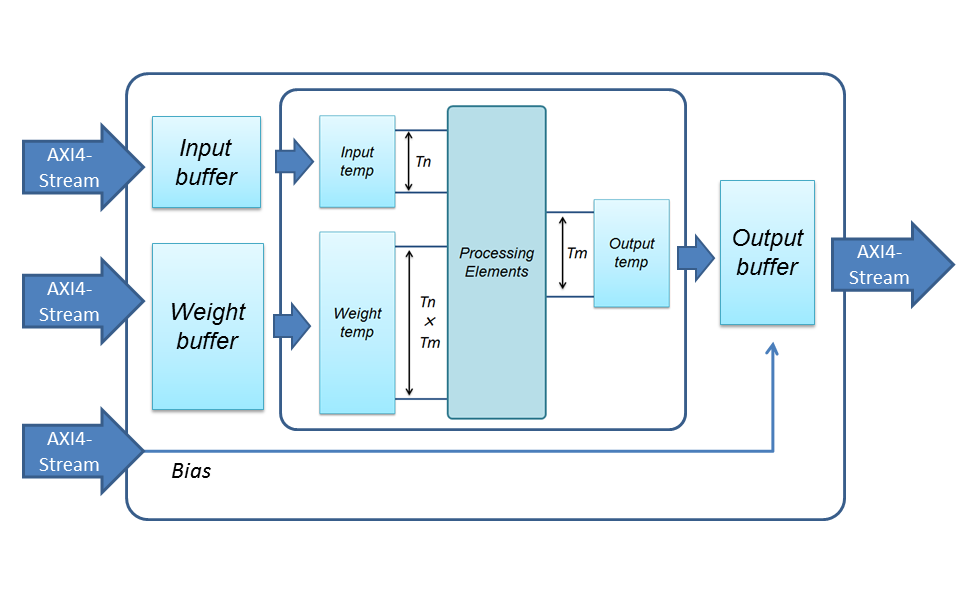
\includegraphics[bb=0 0 720 420, width=1.0\columnwidth]{img/hw.png}
  \caption{アクセラレータの概略図}
%  \ecaption{Static analysis result of an example pattern}
  \label{hw}  
 \end{center}  
\end{figure}

\subsection{演算モジュール}
この節では畳み込み演算の並列性に沿って最適化された演算モジュールを設計する。

図\ref{pe}は今回実装した演算モジュールの概要である。図\ref{fig=conv}のように、畳み込み層の特徴のひとつとして、その多くの処理が入力と重みの積和演算から構成されるという点が挙げられる。
この処理の高速化には複数個の積和演算器を並列に配置するのが最も単純で効率的な方法だと考えられる。
したがって、演算モジュールはTn個の入力値からTn×Tm個の重みを用いてT個の出力値を並列に計算できる汎用的な設計となった。
さらに、スループット向上のためにPE内部はパイプライン化されており、毎サイクルTm個の値を出力バッファへと出力することができる。

パラメータTm、Tnはそれぞれ、演算モジュールが同時に扱う入力データ、出力データの数であり、リソース消費量とトレードオフ関係にあるため実装最適化の対象となる。
今回の設計では暫定的に演算モジュールのサイズは(Tm, Tn)=(24, 8)に固定したが、リソース上限によってはこのパラメータを変更することでリソース上限内に消費量を
抑えることが必要となる。

\begin{figure}[ht]  
 \begin{center}   
   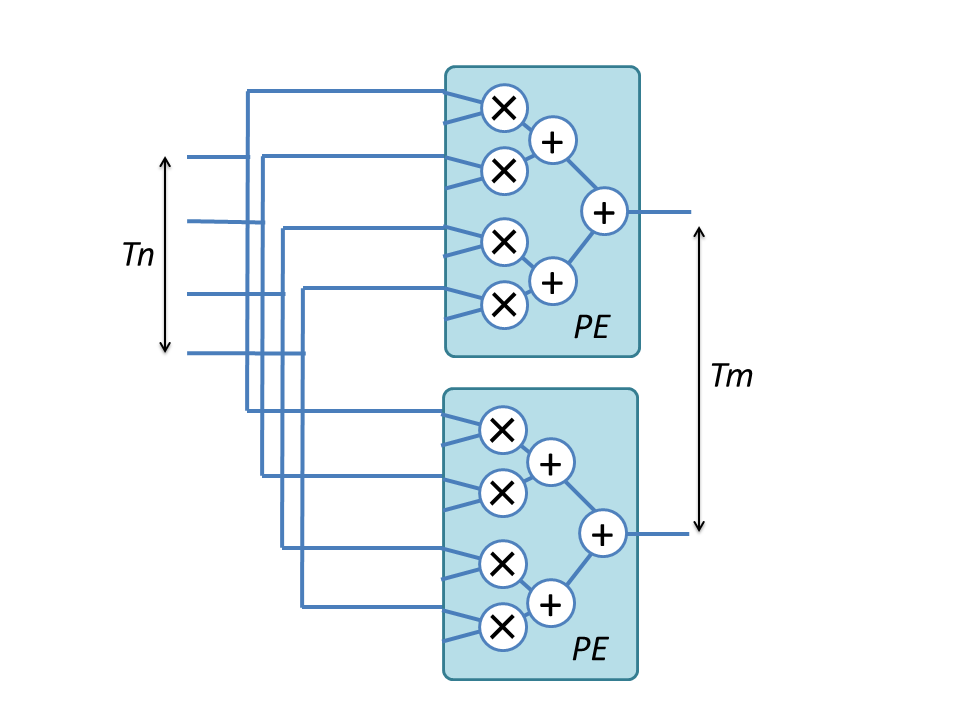
\includegraphics[width=1.0\columnwidth, bb=0 0 720 540]{img/pe.png}
  \caption{Tn×Tm並列の積和を行う演算モジュール}
%  \ecaption{Static analysis result of an example pattern}
  \label{pe}  
 \end{center}  
\end{figure}

\subsection{入出力バッファと重みバッファ}
スイッチモジュールから送られてきた入力特徴マップのデータは、まずFPGA上に確保された入力バッファに蓄えられる。

高速に畳み込み演算を行うためには、演算モジュールは可能な限り広い帯域幅で入力特徴マップにアクセスできなけらばならない。
そこで、入力バッファを特徴マップごとにバンクを分割し並列に読み込むことができるようにした。
これにより、入力バッファと演算モジュールの帯域幅はTn/バンク数となり、帯域幅を改善することができる。

今回の実装では、入力バッファはTn個、出力バッファはTm個、重みバッファはTm×Tn個に分割することで、可能な限り最大の帯域幅を確保した。
これにより、演算モジュールが毎サイクル、畳み込み演算を行う効率的な機構を実現した。
ただし、この実装を行う場合、バンク数に応じてFPGAリソース消費量が増大するため、過剰なバンク分割によってリソースを浪費することに注意しなければならない。


